\clearpage

\section {Validation of the {\em VALOR} Run 5+6  $\bar{\nu}_{\mu}$-disappearance analysis}
\label{sec:validation}

The performance of the fitter was evaluated using ensembles of 3k or 5k toy MC experiments, and these were
generated with statistical fluctuations and variations of all \NSyst{} systematic parameters.
Toy ensembles were generated for both the normal and the inverted mass hierarchies, and were fitted 
using MINUIT and the MINUIT HESSE errors. Distributions of pulls of $\sin^{2}\overline{\theta}_{23}$ 
and $|\overline{\Delta m}^2_{32}|$ are shown in figures~\ref{fig:residuals:oscparams} for both \FakePot{} 
POT and full (\TargetFullPot{}) POT, with true input values of  
$\sin^{2}\overline{\theta}_{23}$ = \NonReactorMixingTwoThreeNH{} and $|\overline{\Delta m}^2_{32}|$ = \NonReactorDmsqNH{}. 
The distributions for $|\overline{\Delta m}^2_{32}|$ are as expected, with a mean close to 0 and a RMS 
that is very near 1.0 for full POT. The tails in the distributions for $\sin^{2}\overline{\theta}_{23}$ are 
caused by toys with upward statistical fluctuations in the bins near the oscillation maximum, which 
are fitted with a value of $\sin^{2}\overline{\theta}_{23}$ that is less than maximal; these best-fit 
values can be in either octant since P($\nu_{\mu} \rightarrow \nu_{\mu}$) is almost identical between a 
value of $\sin^{2}\overline{\theta}_{23}$ and its mirror value in the other octant. The spike near zero 
is due to toys which have either small or downward statistical fluctuations in the bins near the 
oscillation maximum; the spike is smaller at full POT since there are fewer toys with downward statistical 
fluctuations.   

The pulls of $\sin^{2}\overline{\theta}_{23}$ and $|\overline{\Delta m}^2_{32}|$ are also shown in
figures~\ref{fig:pulls_mix23bar_0p35} and~\ref{fig:pulls_dm32sqbar_0p35} from 3k toy MC experiments with input values 
$\sin^{2}\overline{\theta}_{23}$ = 0.35 and $|\overline{\Delta m}^2_{32}|$ = \DmsqNH{}. In these figures, the pulls 
for $|\overline{\Delta m}^2_{32}|$ are as expected, with a mean near 0 and a width that approaches 1.0 at full POT.
The pulls for $\sin^{2}\overline{\theta}_{23}$ appear to have a positive bias at 3.0$\times$10$^{20}$ POT, and 
this is caused by toys with downward statistical fluctuations in bins near the oscillation maximum; these toys 
are fitted with maximal $\sin^{2}\overline{\theta}_{23}$, and this is seen more clearly in the distribution of 
residuals (figure~\ref{fig:residuals_mix23bar_0p35}). The bias disappears at full POT since there are less toys 
with downward statistical fluctuations at higher statistics. Similar distributions are seen in the pulls of 
$\sin^{2}\overline{\theta}_{23}$ and $|\overline{\Delta m}^2_{32}|$ from 3k toys with input values 
$\sin^{2}\overline{\theta}_{23}$ = 0.65 and $|\overline{\Delta m}^2_{32}|$ = \DmsqNH{} in
figures~\ref{fig:pulls_mix23bar_0p65} and~\ref{fig:pulls_dm32sqbar_0p65}; here there appears to be negative bias 
in the pulls of $\sin^{2}\overline{\theta}_{23}$ at 3.0$\times$10$^{20}$ POT, which is again due to downward 
statistical fluctuations in bins near the oscillation maximum and disappears at full POT. 

The pull distributions of these two oscillation parameters are also shown from 3k toys experiments with input values 
$\sin^{2}\overline{\theta}_{23}$ = \NonReactorMixingTwoThreeNH{} and $|\overline{\Delta m}^2_{32}|$ = 2.2$\times$10$^{-3}$ 
eV$^{2}$/c$^{4}$ in figures~\ref{fig:pulls_mix23bar_0p0022} and~\ref{fig:pulls_dm32sqbar_0p0022} and from 3k toys 
with input values $\sin^{2}\overline{\theta}_{23}$ = \NonReactorMixingTwoThreeNH{} and $|\overline{\Delta m}^2_{32}|$ = 
2.8$\times$10$^{-3}$ eV$^{2}$/c$^{4}$ in figures~\ref{fig:pulls_mix23bar_0p0028} and~\ref{fig:pulls_dm32sqbar_0p0028}. 
These pull distributions are as expected except that there are small biases of +0.25 and -0.13 in the pull means when the 
input value of $|\overline{\Delta m}^2_{32}|$ is 2.2$\times$10$^{-3}$ eV$^{2}$/c$^{4}$ and 2.8$\times$10$^{-3}$ eV$^{2}$/c$^{4}$ 
respectively for $3 \times 10E{20}$ POT; these biases are reduced to +0.23 and -0.08 respectively for \TargetFullPot{} POT.   
 
%
% Osc param residuals
% 

\begin{figure*}[htb]
 \centering
 \begin{subfigure}[b]{0.70\textwidth}
  \center
  \includegraphics[width=\textwidth]{{./images/fit_bias/pulls_rethrown/pull_mixing23bar}.eps}
  \label{fig:residuals:oscparams:mixing}
  \caption{$\sin^{2}\overline{\theta}_{23}$}
 \end{subfigure}

 \hfill \break

 \begin{subfigure}[b]{0.70\textwidth}
  \center
  \includegraphics[width=\textwidth]{{./images/fit_bias/pulls_rethrown/pull_dmsq23bar}.eps}
  \label{fig:residuals:oscparams:dmsq}
  \caption{$|\overline{\Delta m}^2_{32}|$}
 \end{subfigure}
 \caption {
      Distributions of pulls of $\sin^{2}\overline{\theta}_{23}$ and $|\overline{\Delta m}^2_{32}|$ from 5k toy MC experiments,
      generated at $\sin^{2}\overline{\theta}_{23}$ = \MixingTwoThreeNH{}
      and $|\overline{\Delta m}^2_{32}|$ = \DmsqNH{},
      including statistical fluctuations and with randomised systematic parameters.
      The other oscillation parameters are fixed to the values in Tab.~\ref{tab:osc_params_fixed_values_non_reactor}, and the normal mass hierarchy is assumed.
      The distribution is shown for both
      \FakePot{} POT (Runs 5 and 6, black histogram) and \TargetFullPot{} POT (the T2K ultimate goal,
      red histogram).
  }
  \label{fig:residuals:oscparams}
\end{figure*}

\begin{figure*}[htb]
\begin{minipage}[t]{0.48\linewidth}
\center
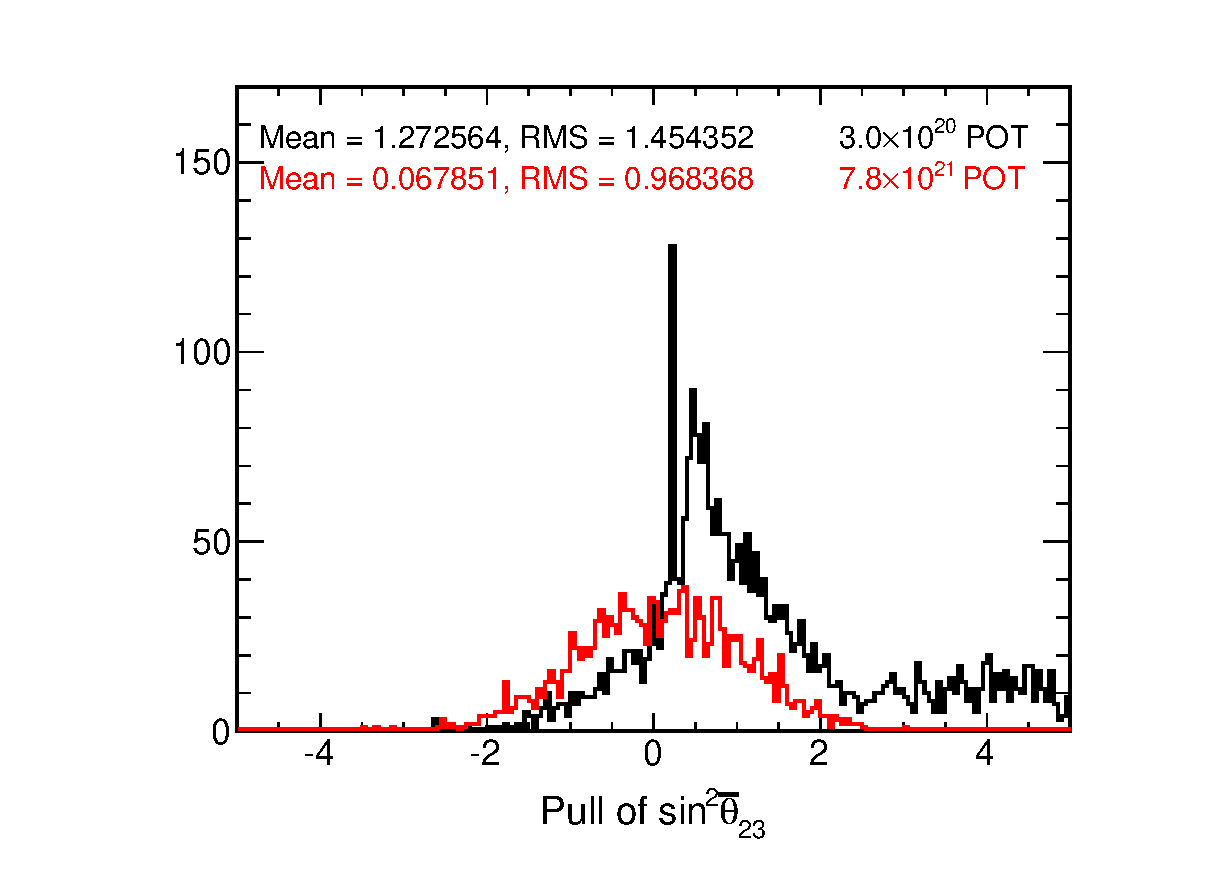
\includegraphics[width=20pc]{./images/fit_bias/pulls_osc_params_3E20/Pull_mixing23bar_0p35.eps}
\caption {
      Distributions of pulls of $\sin^{2}\overline{\theta}_{23}$ from 3k toy MC experiments,
      generated at $\sin^{2}\overline{\theta}_{23}$ = 0.35
      and $|\overline{\Delta m}^2_{32}|$ = \DmsqNH{},
      including statistical fluctuations and with randomised systematic parameters.
      The other oscillation parameters are fixed to the values in Tab.~\ref{tab:osc_params_fixed_values_non_reactor}, and the normal mass hierarchy is assumed.
      The distribution is shown for both
      3.0$\times$10$^{20}$ POT (black histogram) and \TargetFullPot{} POT (the T2K ultimate goal,
      red histogram).
}
\label{fig:pulls_mix23bar_0p35}
\end{minipage}
\hspace{0.06\linewidth}
\begin{minipage}[t]{0.48\linewidth}
\center
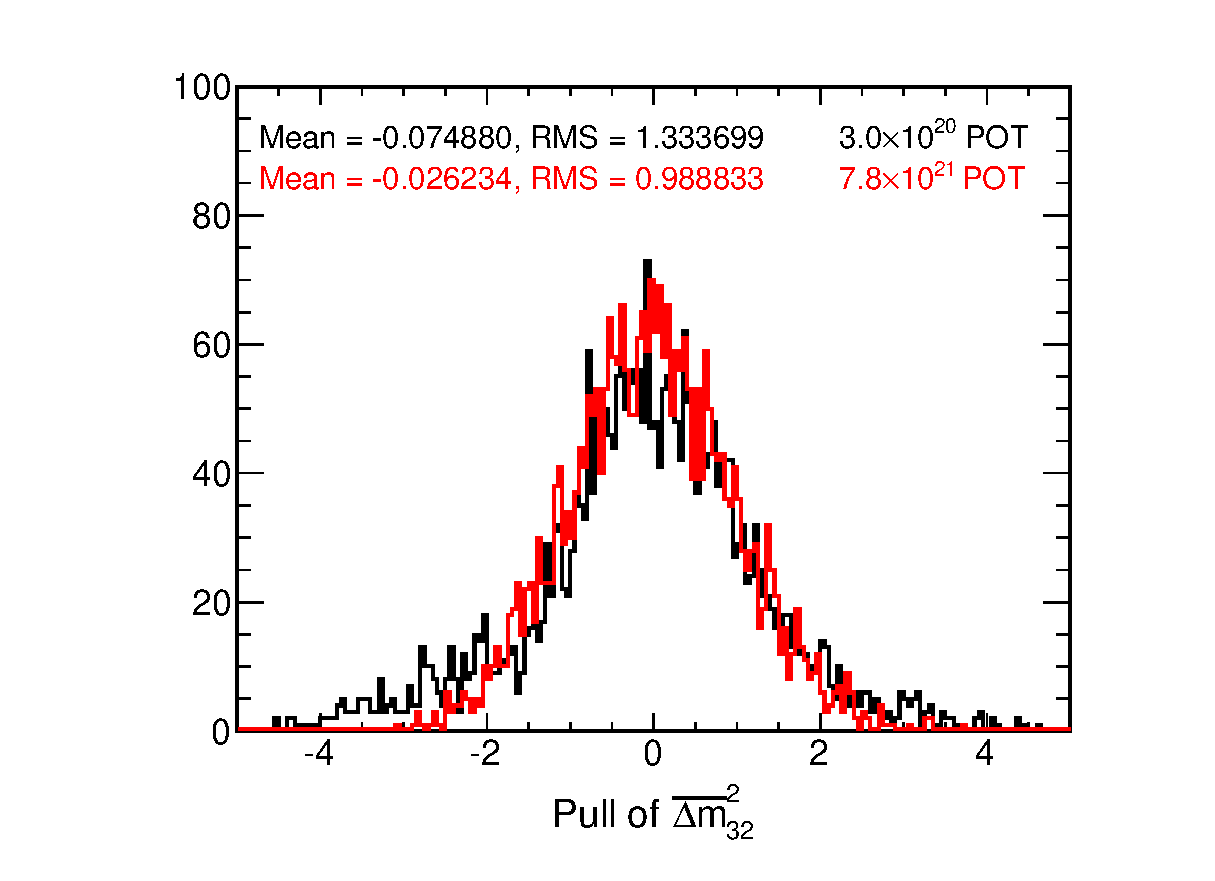
\includegraphics[width=20pc]{./images/fit_bias/pulls_osc_params_3E20/Pull_dm32sqbar_0p35.eps}
\caption {
      Distributions of pulls of $|\overline{\Delta m}^2_{32}|$ from 3k toy MC experiments,
      generated at $\sin^{2}\overline{\theta}_{23}$ = 0.35
      and $|\overline{\Delta m}^2_{32}|$ = \DmsqNH{},
      including statistical fluctuations and with randomised systematic parameters.
      The other oscillation parameters are fixed to the values in Tab.~\ref{tab:osc_params_fixed_values_non_reactor}, and the normal mass hierarchy is assumed.
      The distribution is shown for both
      3.0$\times$10$^{20}$ POT (black histogram) and \TargetFullPot{} POT (the T2K ultimate goal,
      red histogram).
}
\label{fig:pulls_dm32sqbar_0p35}
\end{minipage}
\end{figure*}

\begin{figure*}[htb]
\center
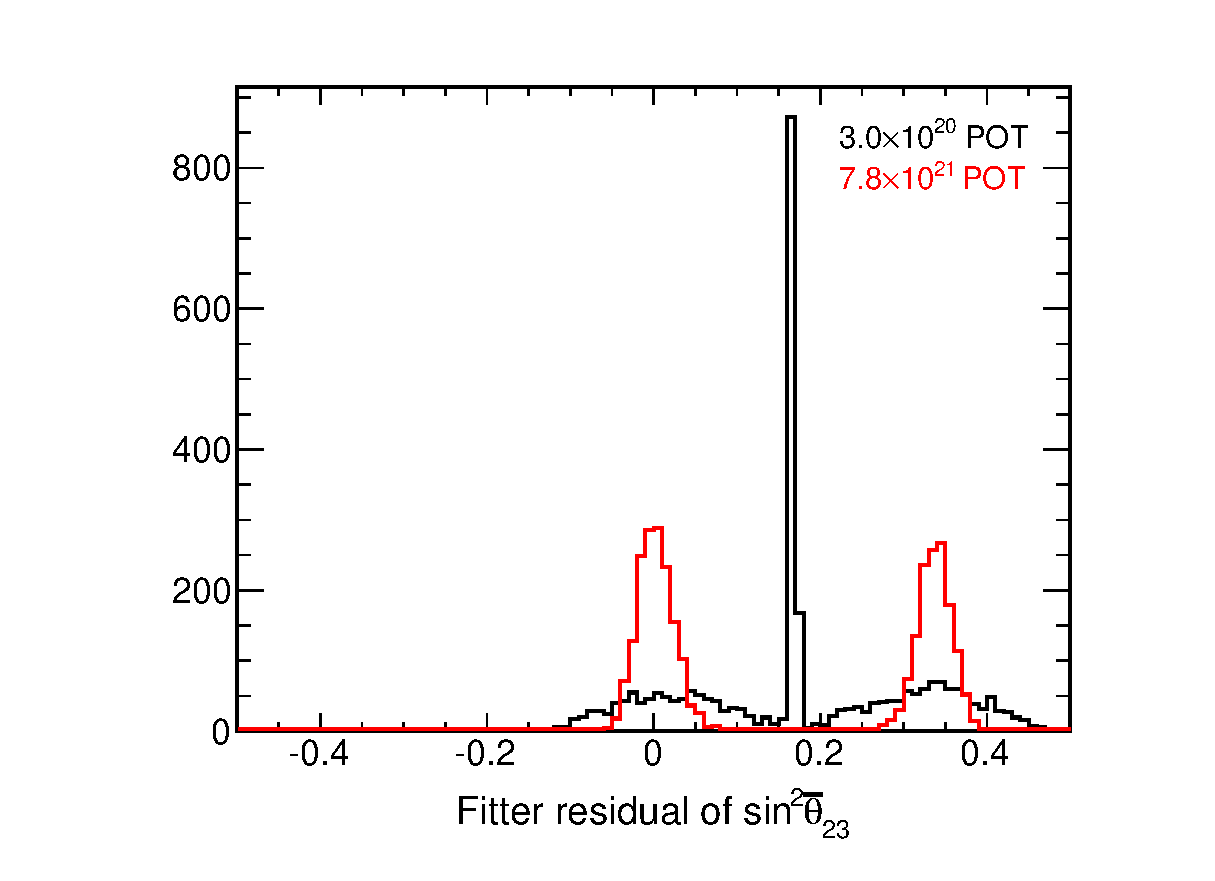
\includegraphics[width=20pc]{./images/fit_bias/pulls_osc_params_3E20/Residual_mixing23bar_0p35.eps}
\caption {
      Distributions of fitter residuals of $\sin^{2}\overline{\theta}_{23}$ from 3k toy MC experiments,
      generated at $\sin^{2}\overline{\theta}_{23}$ = 0.35
      and $|\overline{\Delta m}^2_{32}|$ = \DmsqNH{},
      including statistical fluctuations and with randomised systematic parameters.
      The other oscillation parameters are fixed to the values in Tab.~\ref{tab:osc_params_fixed_values_non_reactor}, and the normal mass hierarchy is assumed.
      The distribution is shown for both
      3.0$\times$10$^{20}$ POT (black histogram) and \TargetFullPot{} POT (the T2K ultimate goal,
      red histogram).
}
\label{fig:residuals_mix23bar_0p35}
\end{figure*}

\begin{figure*}[htb]
\begin{minipage}[t]{0.48\linewidth}
\center
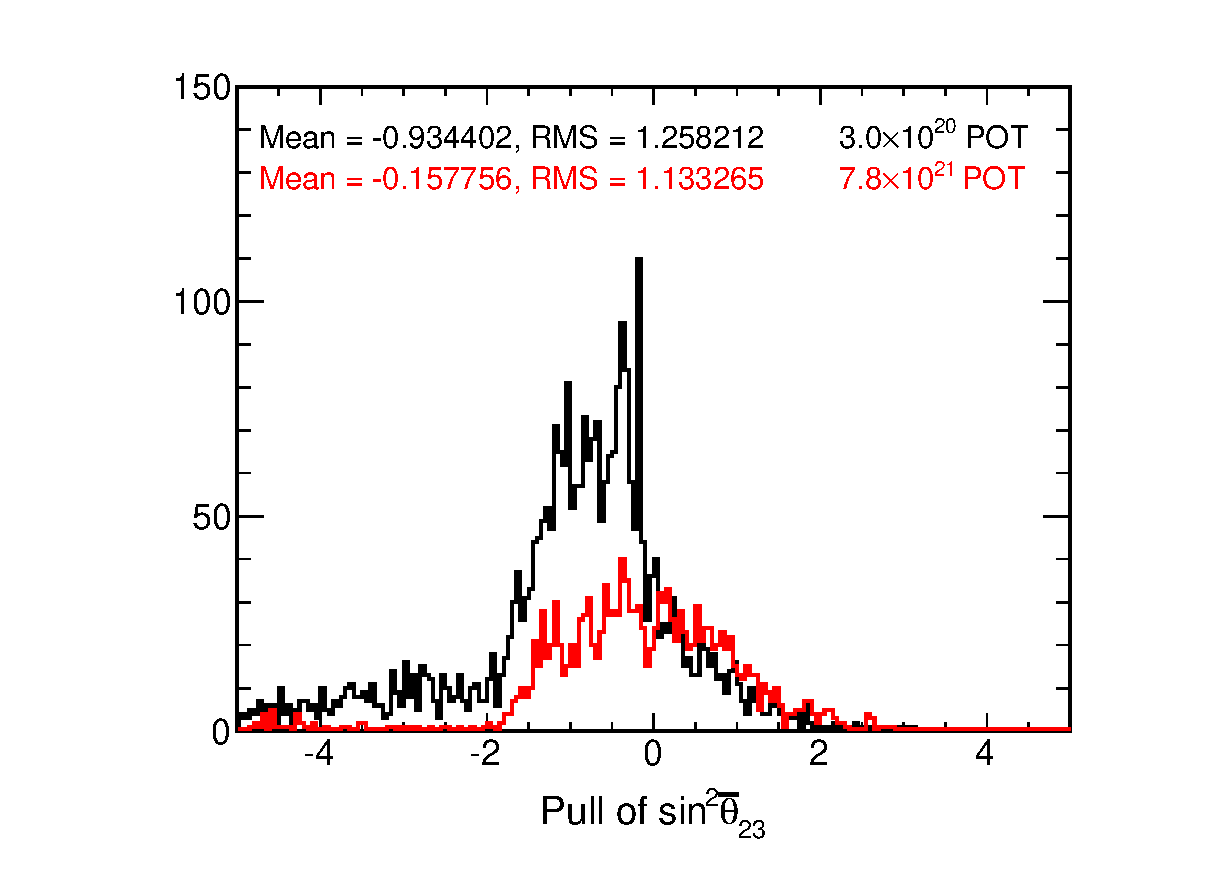
\includegraphics[width=20pc]{./images/fit_bias/pulls_osc_params_3E20/Pull_mixing23bar_0p65.eps}
\caption {
      Distributions of pulls of $\sin^{2}\overline{\theta}_{23}$ from 3k toy MC experiments,
      generated at $\sin^{2}\overline{\theta}_{23}$ = 0.65
      and $|\overline{\Delta m}^2_{32}|$ = \DmsqNH{},
      including statistical fluctuations and with randomised systematic parameters.
      The other oscillation parameters are fixed to the values in Tab.~\ref{tab:osc_params_fixed_values_non_reactor}, and the normal mass hierarchy is assumed.
      The distribution is shown for both
      3.0$\times$10$^{20}$ POT (black histogram) and \TargetFullPot{} POT (the T2K ultimate goal,
      red histogram).
}
\label{fig:pulls_mix23bar_0p65}
\end{minipage}
\hspace{0.06\linewidth}
\begin{minipage}[t]{0.48\linewidth}
\center
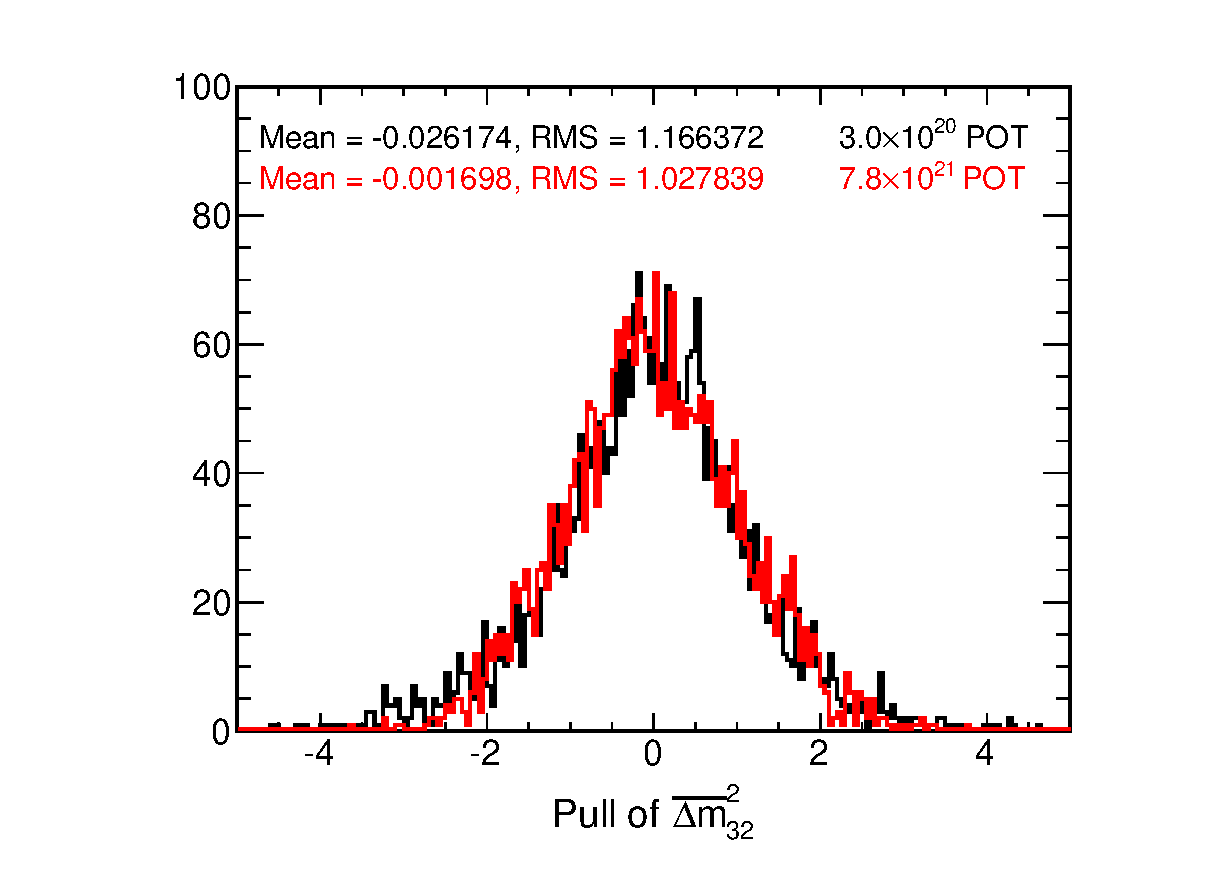
\includegraphics[width=20pc]{./images/fit_bias/pulls_osc_params_3E20/Pull_dm32sqbar_0p65.eps}
\caption {
      Distributions of pulls of $|\overline{\Delta m}^2_{32}|$ from 3k toy MC experiments,
      generated at $\sin^{2}\overline{\theta}_{23}$ = 0.65
      and $|\overline{\Delta m}^2_{32}|$ = \DmsqNH{},
      including statistical fluctuations and with randomised systematic parameters.
      The other oscillation parameters are fixed to the values in Tab.~\ref{tab:osc_params_fixed_values_non_reactor}, and the normal mass hierarchy is assumed.
      The distribution is shown for both
      3.0$\times$10$^{20}$ POT (black histogram) and \TargetFullPot{} POT (the T2K ultimate goal,
      red histogram).
}
\label{fig:pulls_dm32sqbar_0p65}
\end{minipage}
\end{figure*}

\begin{figure*}[htb]
\center
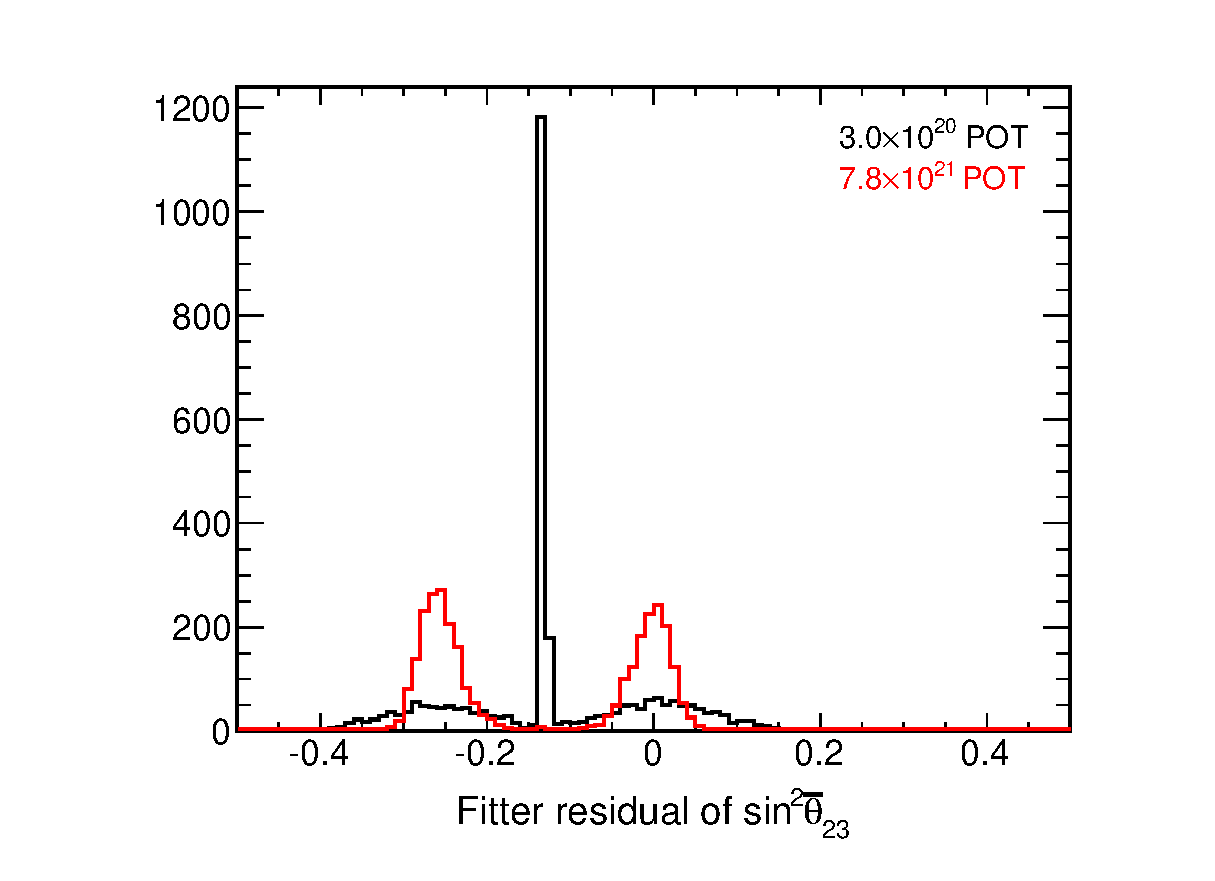
\includegraphics[width=20pc]{./images/fit_bias/pulls_osc_params_3E20/Residual_mixing23bar_0p65.eps}
\caption {
      Distributions of fitter residuals of $\sin^{2}\overline{\theta}_{23}$ from 3k toy MC experiments,
      generated at $\sin^{2}\overline{\theta}_{23}$ = 0.65
      and $|\overline{\Delta m}^2_{32}|$ = \DmsqNH{},
      including statistical fluctuations and with randomised systematic parameters.
      The other oscillation parameters are fixed to the values in Tab.~\ref{tab:osc_params_fixed_values_non_reactor}, and the normal mass hierarchy is assumed.
      The distribution is shown for both
      3.0$\times$10$^{20}$ POT (black histogram) and \TargetFullPot{} POT (the T2K ultimate goal,
      red histogram).
}
\label{fig:residuals_mix23bar_0p65}
\end{figure*}

\begin{figure*}[htb]
\begin{minipage}[t]{0.48\linewidth}
\center
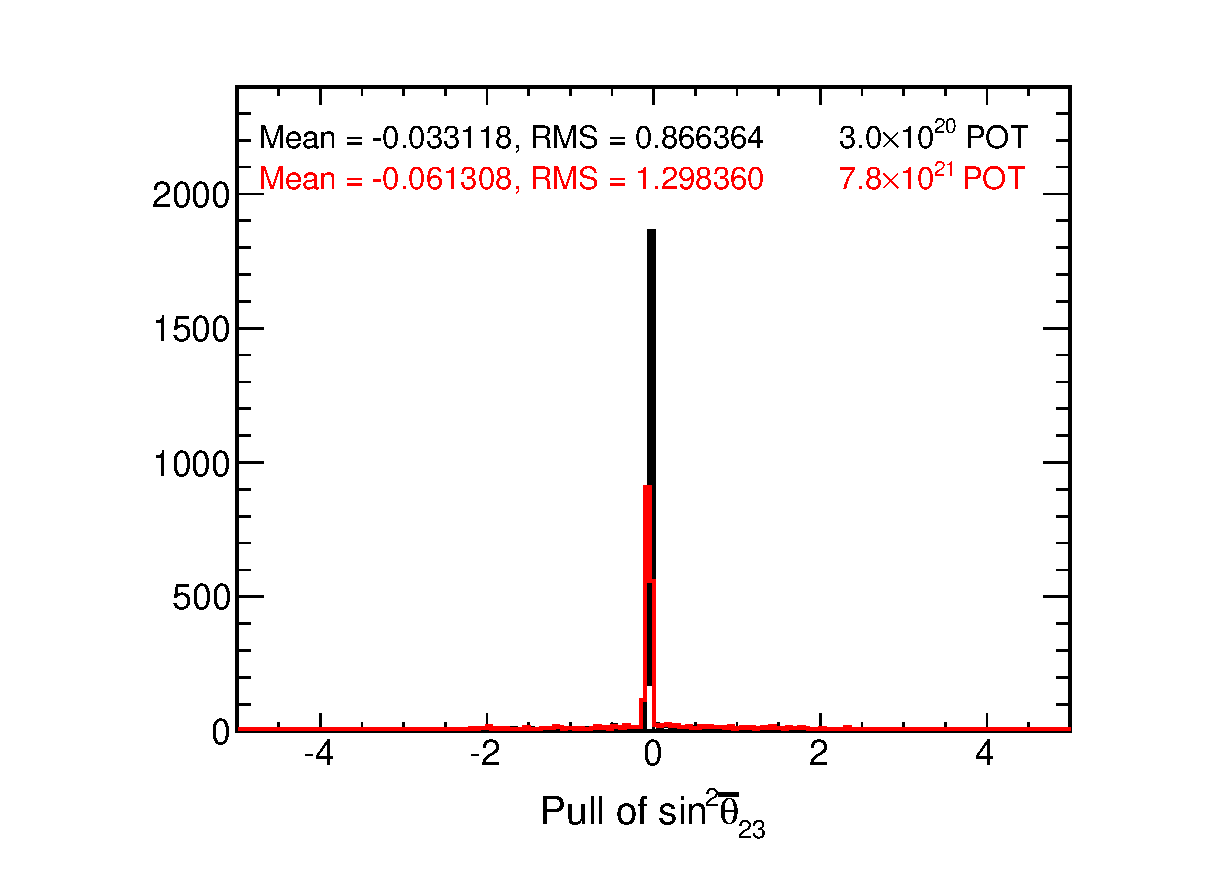
\includegraphics[width=20pc]{./images/fit_bias/pulls_osc_params_3E20/Pull_mixing23bar_0p0022.eps}
\caption {
      Distributions of pulls of $\sin^{2}\overline{\theta}_{23}$ from 3k toy MC experiments,
      generated at $\sin^{2}\overline{\theta}_{23}$ = 0.524
      and $|\overline{\Delta m}^2_{32}|$ = 2.2$\times$10$^{-3}$eV$^{2}$/c$^{4}$,
      including statistical fluctuations and with randomised systematic parameters.
      The other oscillation parameters are fixed to the values in Tab.~\ref{tab:osc_params_fixed_values_non_reactor}, and the normal mass hierarchy is assumed.
      The distribution is shown for both
      3.0$\times$10$^{20}$ POT (black histogram) and \TargetFullPot{} POT (the T2K ultimate goal,
      red histogram).
}
\label{fig:pulls_mix23bar_0p0022}
\end{minipage}
\hspace{0.06\linewidth}
\begin{minipage}[t]{0.48\linewidth}
\center
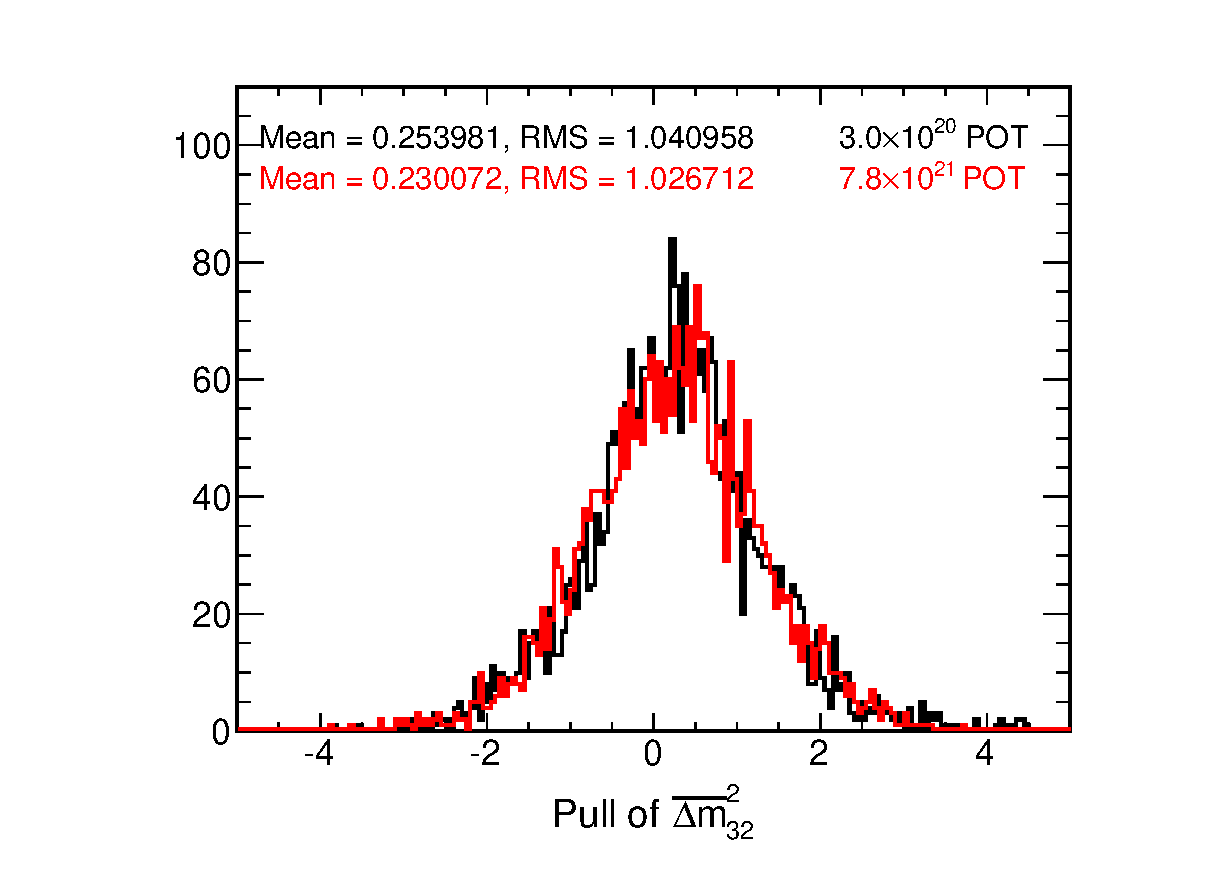
\includegraphics[width=20pc]{./images/fit_bias/pulls_osc_params_3E20/Pull_dm32sqbar_0p0022.eps}
\caption {
      Distributions of pulls of $|\overline{\Delta m}^2_{32}|$ from 3k toy MC experiments,
      generated at $\sin^{2}\overline{\theta}_{23}$ = 0.524
      and $|\overline{\Delta m}^2_{32}|$ = 2.2$\times$10$^{-3}$eV$^{2}$/c$^{4}$,
      including statistical fluctuations and with randomised systematic parameters.
      The other oscillation parameters are fixed to the values in Tab.~\ref{tab:osc_params_fixed_values_non_reactor}, and the normal mass hierarchy is assumed.
      The distribution is shown for both
      3.0$\times$10$^{20}$ POT (black histogram) and \TargetFullPot{} POT (the T2K ultimate goal,
      red histogram).
}
\label{fig:pulls_dm32sqbar_0p0022}
\end{minipage}
\end{figure*}

\begin{figure*}[htb]
\begin{minipage}[t]{0.48\linewidth}
\center
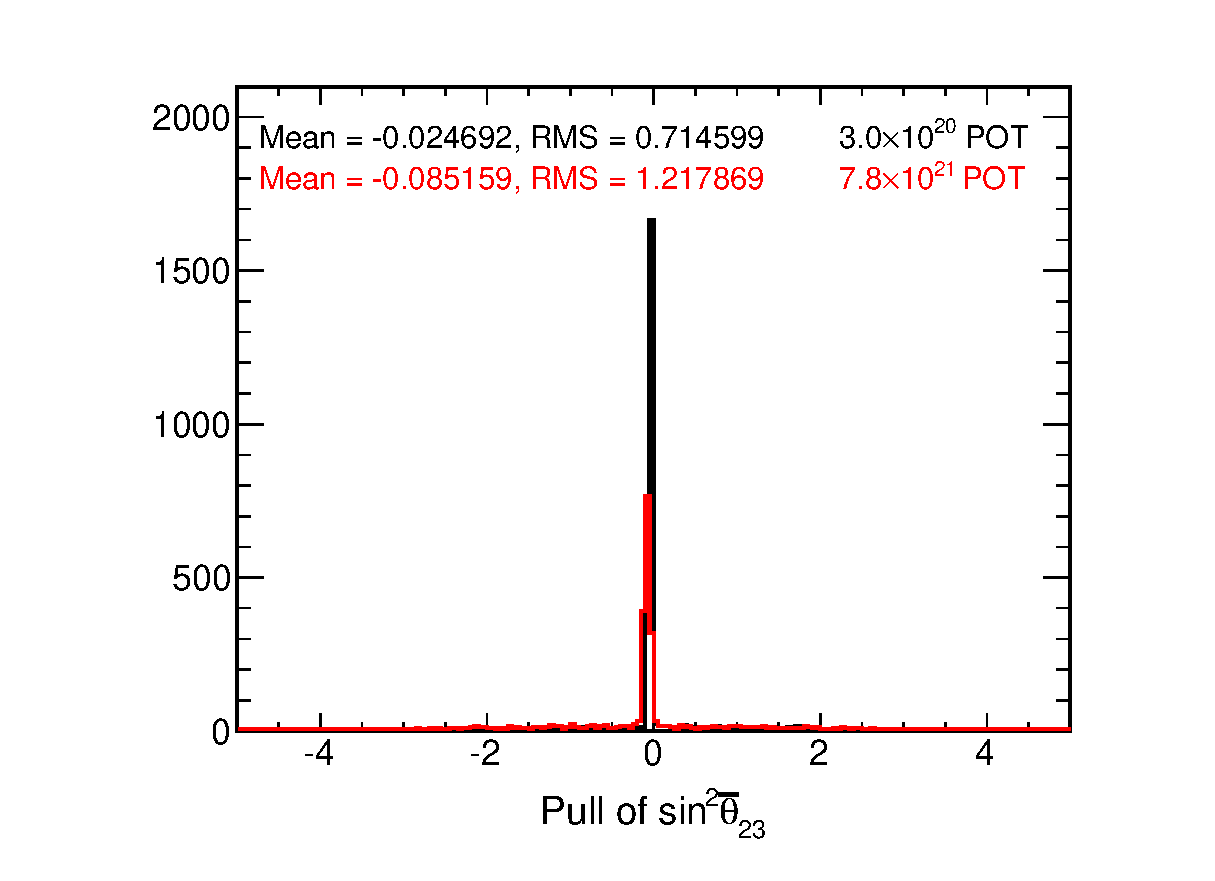
\includegraphics[width=20pc]{./images/fit_bias/pulls_osc_params_3E20/Pull_mixing23bar_0p0028.eps}
\caption {
      Distributions of pulls of $\sin^{2}\overline{\theta}_{23}$ from 3k toy MC experiments,
      generated at $\sin^{2}\overline{\theta}_{23}$ = 0.524
      and $|\overline{\Delta m}^2_{32}|$ = 2.8$\times$10$^{-3}$eV$^{2}$/c$^{4}$,
      including statistical fluctuations and with randomised systematic parameters.
      The other oscillation parameters are fixed to the values in Tab.~\ref{tab:osc_params_fixed_values_non_reactor}, and the normal mass hierarchy is assumed.
      The distribution is shown for both
      3.0$\times$10$^{20}$ POT (black histogram) and \TargetFullPot{} POT (the T2K ultimate goal,
      red histogram).
}
\label{fig:pulls_mix23bar_0p0028}
\end{minipage}
\hspace{0.06\linewidth}
\begin{minipage}[t]{0.48\linewidth}
\center
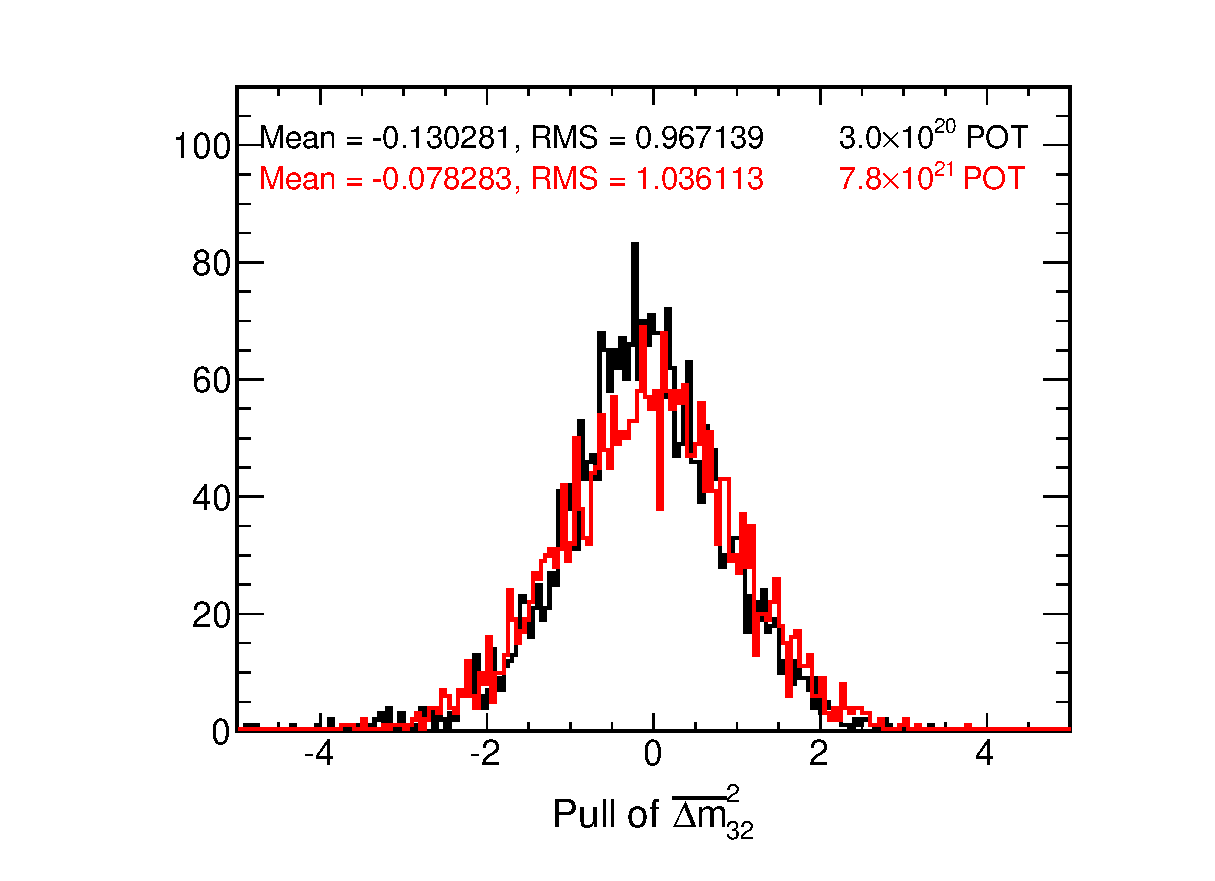
\includegraphics[width=20pc]{./images/fit_bias/pulls_osc_params_3E20/Pull_dm32sqbar_0p0028.eps}
\caption {
      Distributions of pulls of $|\overline{\Delta m}^2_{32}|$ from 3k toy MC experiments,
      generated at $\sin^{2}\overline{\theta}_{23}$ = 0.524
      and $|\overline{\Delta m}^2_{32}|$ = 2.8$\times$10$^{-3}$eV$^{2}$/c$^{4}$,
      including statistical fluctuations and with randomised systematic parameters.
      The other oscillation parameters are fixed to the values in Tab.~\ref{tab:osc_params_fixed_values_non_reactor}, and the normal mass hierarchy is assumed.
      The distribution is shown for both
      3.0$\times$10$^{20}$ POT (black histogram) and \TargetFullPot{} POT (the T2K ultimate goal,
      red histogram).
}
\label{fig:pulls_dm32sqbar_0p0028}
\end{minipage}
\end{figure*}


A check was also made of the pull distributions of the systematic parameters, and, in these studies, two different types 
of systematic parameter throws were used: in one set of fits, systematic parameter throws were restricted to physically-allowed values,
and were rethrown if a thrown value was outside these limits. Thus the throw distribution formed a truncated Gaussian.
In the second set of fits, throws of systematic parameters were allowed to be outside their physical limits,
leading to a full Gaussian distribution of thrown values.

A summary of the mean and RMS of pulls from the unrestricted fits can be seen
in figures~\ref{fig:validation_pulls_normal_no_rethrow}
and~\ref{fig:validation_pulls_inverted_no_rethrow}.
No problems were identified with the fitter, which performed as expected, and there are only small deviations 
from the expected mean of 0 and RMS of 1.

% Pulls figures - with parameters not rethrown
\begin{figure*}[htb]
  \center
  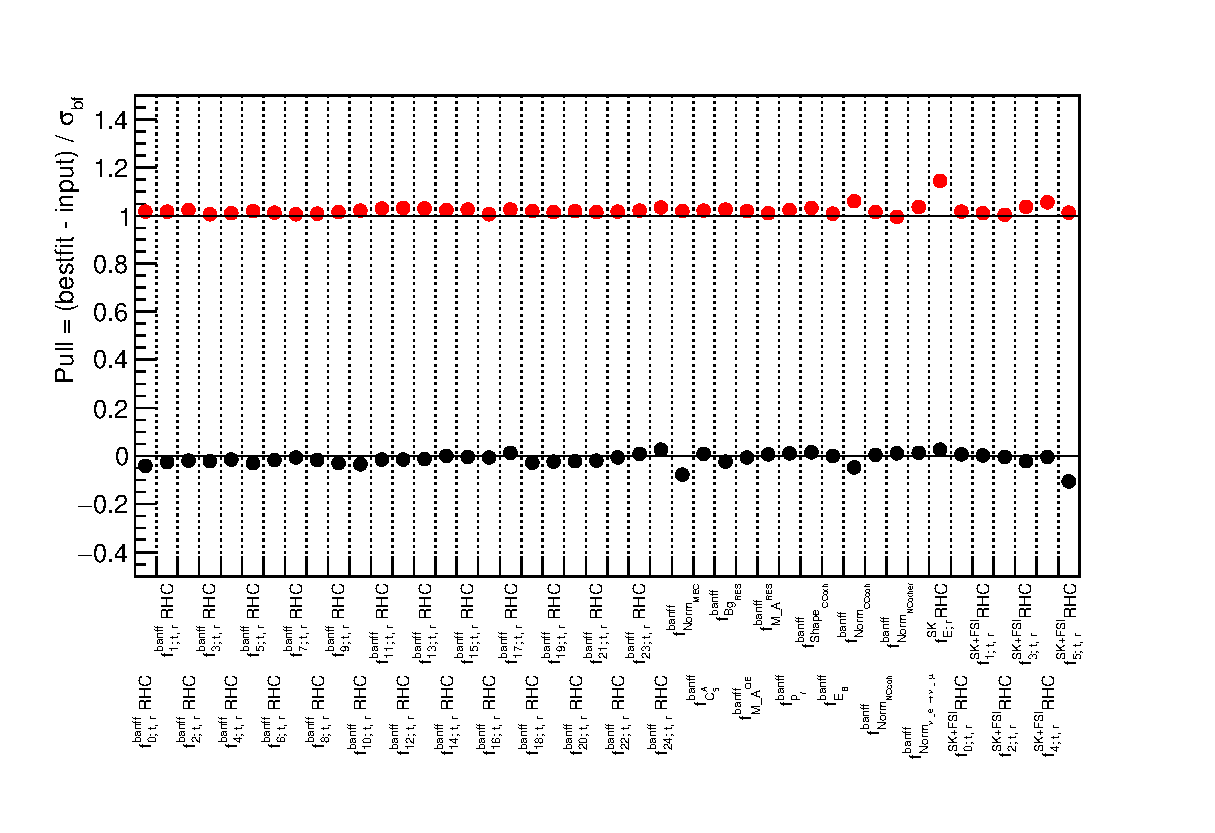
\includegraphics[width=50pc,angle=270]{./images/fit_bias/normal_2p5E20_no_rethrow_pulls.eps}
  \caption {
    Summary of systematic pull distributions for all systematic parameters for
    5k toy MC experiments at \FakePot{} POT 
    including statistical fluctuations and with randomised systematic parameters.
    Throws of systematic parameters were allowed to be thrown outside the physical region.
    All other oscillation parameters were fixed at their values from table~\ref{tab:osc_params_fixed_values_non_reactor}.
    The normal mass hierarchy is assumed.
  }
  \label{fig:validation_pulls_normal_no_rethrow}
\end{figure*}

\begin{figure*}[htb]
  \center
  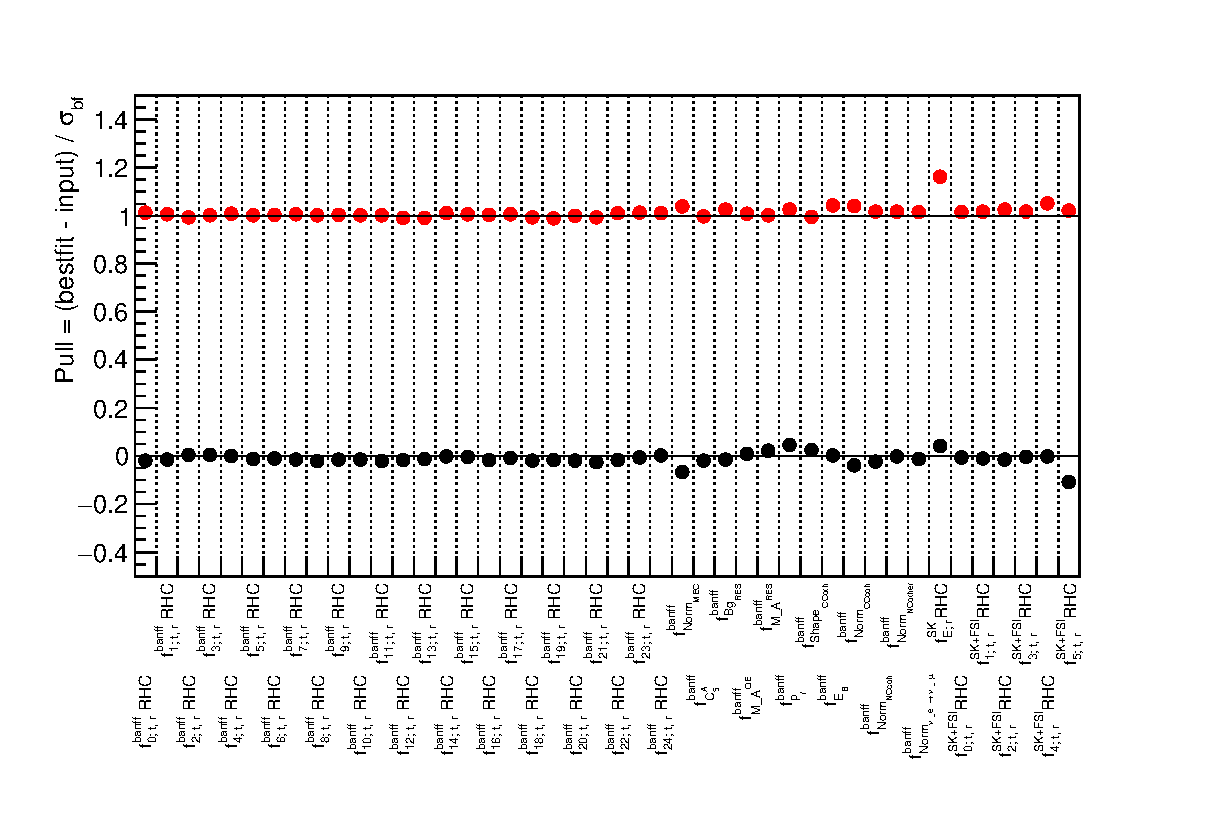
\includegraphics[width=50pc,angle=270]{./images/fit_bias/inverted_2p5E20_no_rethrow_pulls.eps}
  \caption {
    Summary of systematic pull distributions for all systematic parameters for
    5k toy MC experiments at \FakePot{} POT 
    including statistical fluctuations and with randomised systematic parameters.
    Throws of systematic parameters were allowed to be thrown outside the physical region.
    All other oscillation parameters were fixed at their values from table~\ref{tab:osc_params_fixed_values_non_reactor}.
    The inverted mass hierarchy is assumed.
  }
  \label{fig:validation_pulls_inverted_no_rethrow}
\end{figure*}

% Pulls figures - with parameters rethrown
\begin{figure*}[htb]
  \center
  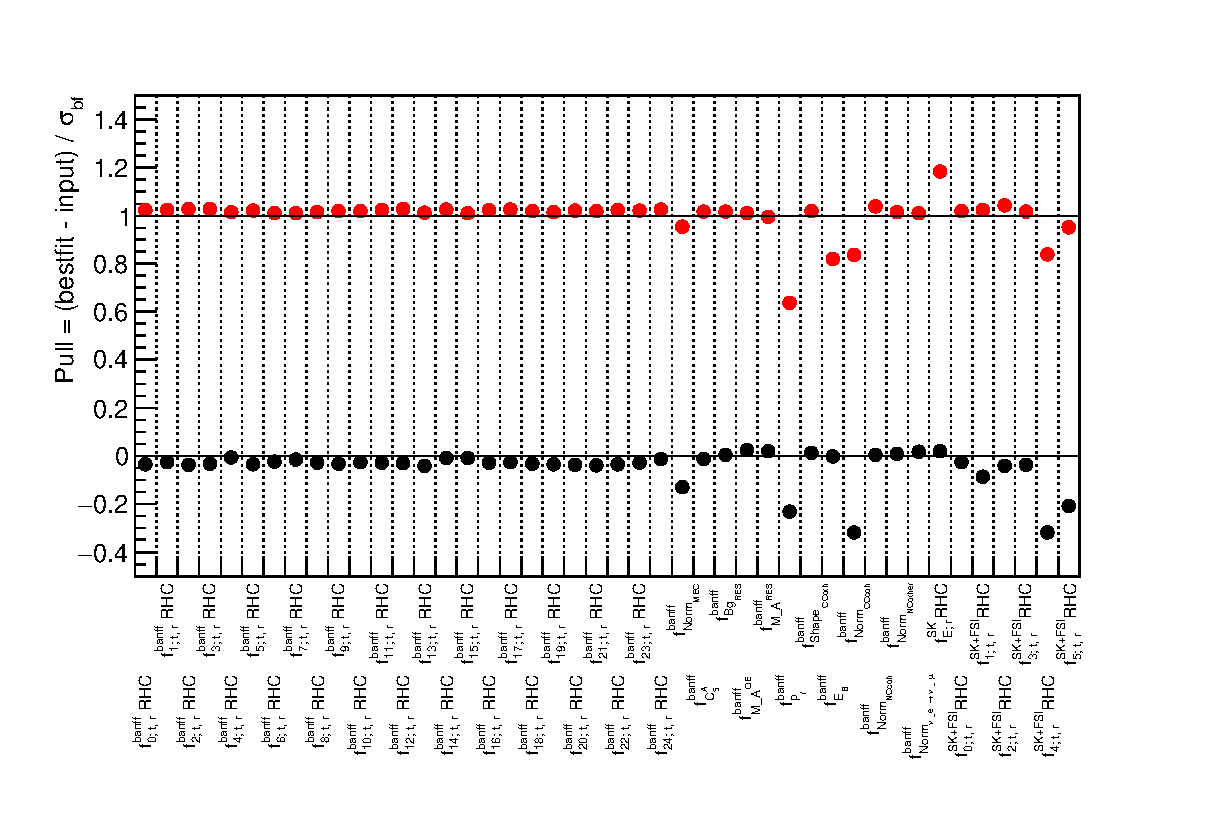
\includegraphics[width=50pc,angle=270]{./images/fit_bias/normal_2p5E20_rethrow_pulls.eps}
  \caption {
    Summary of systematic pull distributions for all systematic parameters for
    5k toy MC experiments at \FakePot{} POT 
    including statistical fluctuations and with randomised systematic parameters.
    Systematic parameters were rethrown if an unphysical thrown value was obtained.
    All other oscillation parameters were fixed at their values from table~\ref{tab:osc_params_fixed_values_non_reactor}.
    The normal mass hierarchy is assumed.
  }
  \label{fig:validation_pulls_normal_rethrow}
\end{figure*}

\begin{figure*}[htb]
  \center
  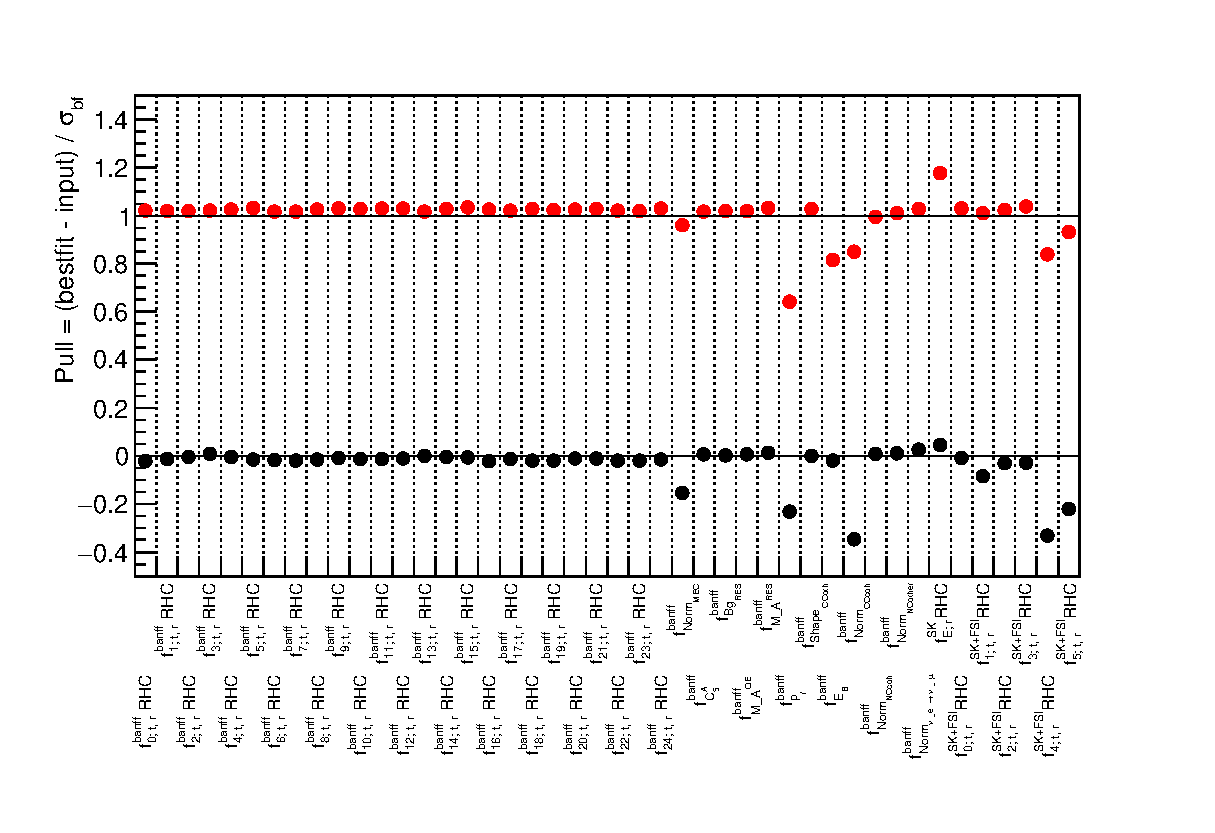
\includegraphics[width=50pc,angle=270]{./images/fit_bias/inverted_2p5E20_rethrow_pulls.eps}
  \caption {
    Summary of systematic pull distributions for all systematic parameters for
    5k toy MC experiments at \FakePot{} POT 
    including statistical fluctuations and with randomised systematic parameters.
    Systematic parameters were rethrown if an unphysical thrown value was obtained.
    All other oscillation parameters were fixed at their values from table~\ref{tab:osc_params_fixed_values_non_reactor}.
    The inverted mass hierarchy is assumed.
  }
  \label{fig:validation_pulls_inverted_rethrow}
\end{figure*}

Pulls for the restricted fits can be seen in figure~\ref{fig:validation_pulls_normal_rethrow}
and~\ref{fig:validation_pulls_inverted_rethrow}. These pulls are Gaussian with mean 1 and RMS 0 for most systematic parameters, 
but show small differences from this for a few parameters. The differences from a Gaussian with mean 0 and RMS 1 for these parameters 
are understood:
\begin{itemize}
\item {\bf SuperK energy scale.}
  This systematic is different from the others in that it migrates events from bin to bin instead of increasing or decreasing the 
  numbers of events in the bins of reconstructed energy. Its pull is not expected to be a Gaussian with zero mean since the shape 
  of the predicted energy spectrum is not symmetric, and, consequently, a positive tweak of this parameter has a 
  different effect on that spectrum from a negative tweak.
  This can lead to a discontinuity in the derivative of the $\chi^2$ distribution
  at the zero point, which also contributes to a larger number of fits with this best-fit point.
  An example of this discontinuity can be seen in figure~\ref{fig:energy_scale_chisquare_discontinuity}.
\item {\bf Fermi Momentum.}
  This systematic has a physical limit between 200 MeV and 275 MeV.
  The unconstrained parameter value is 225 MeV and the 1$\sigma$ error is 31 MeV.
  Consequently, the parameter has physical limits at around -1 and +2$\sigma$.
  The fitter cannot reach the true values when the parameter is thrown beyond these limits.
  The asymmetry of the allowed region around the central value results in a small downward bias in the pulls.
%  A distribution of the restricted throws can be seen in figure\ref{NOSUCHFIGURE}.
\item {\bf MEC Normalisation}
  The MEC normalisation on $^{16}$O has a nominal value of 1.0 and a prefit error of 73.3\%. This means that some unrestricted throws of 
  this parameter are $<$ 0, which is unphysical. Hence the restricted throws have a Gaussian distribution that is truncated at its lower 
  end. The throw values that are truncated are the lowest values, and these would be expected to have positive pulls due to the penalty 
  term pulling them towards the nominal value. This leads to a pull distribution that is narrower on the plus side than on the minus side.    
\item {\bf CC Coherent Normalisation}
  The CC coherent normalisation has a nominal value of 1.0 and a prefit error of 100\%. This means that some unrestricted throws of
  this parameter are $<$ 0, which is unphysical. Hence the restricted throws have a Gaussian distribution that is truncated at its lower
  end. The throw values that are truncated are the lowest values, and these would be expected to have positive pulls due to the penalty
  term pulling them towards the nominal value. This leads to a pull distribution that is narrower on the plus side than on the minus side.
\item {\bf SuperK Detector + FSI + SI Parameter 6 (all NC events)}
%  The physical limit of a normalisation parameter is at zero.
%  The NC contribution to the muon-like sample is tiny, and the error on this quantity is large.
%  This makes the physical limit important again.
%  As can be seen in table~\ref{tab:star_plot}, the effect of systematic is negligible.
% \item {\bf NC SuperK detector efficiency + FSI + SI.} 
   The bias comes from the low statistics at \FakePot{} POT.
   When Poisson fluctuations are made of the bin contents of the $E_{reco}$ distributions, a downward fluctuation is more likely than an upward
   fluctuation. For example, a Poisson distribution with mean 3 has P(1) = 0.149 and P(2) = 0.224, whereas P(4) = 0.168 and P(5) = 0.101. The 
   NC events are mainly around the oscillation maximum where there are few events, and downward Poisson fluctuations are more likely than upward 
   ones. Fitting these downward fluctuations involves moving this parameter down from zero, and this explains the negative bias in its pull. 
  %~ When moving away from the point of maximal disappearance as input
  %~ (and so reducing the depth of the oscillation dip),
  %~ the NC bin in the SuperK detector efficiency + FSI + SI matrix bias is reduced.
\end{itemize}
The pull distributions for four of the systematics with biases are shown in figures~\ref{fig:residuals:badsystematics}.

%
% Biased syst param pulls
% 

\begin{figure*}[htb]
 \centering
 \begin{subfigure}[b]{0.45\textwidth}
  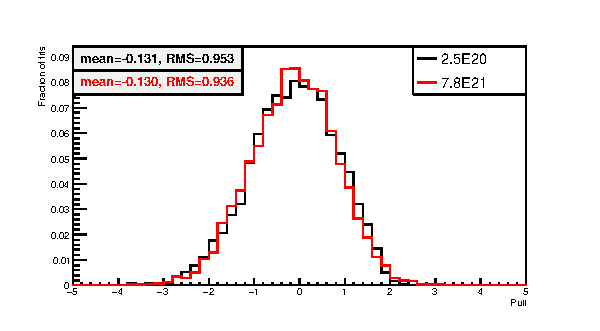
\includegraphics[width=\textwidth]{./images/fit_bias/pulls_rethrown/pull_f_banffmec_rhc.eps}
  \label{fig:residuals:mec}
  \caption{MEC Normalisation on $^{16}$O}
 \end{subfigure}
 %
 \begin{subfigure}[b]{0.45\textwidth}
  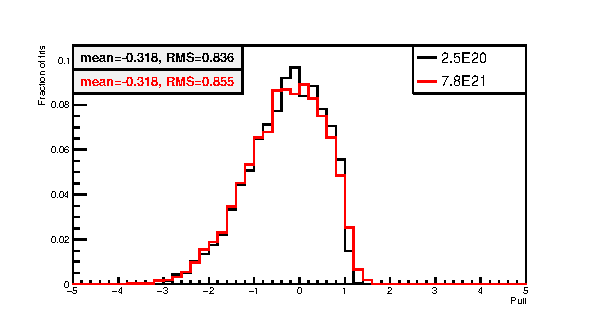
\includegraphics[width=\textwidth]{./images/fit_bias/pulls_rethrown/pull_f_banffnorm_cccoh_rhc.eps}
  \label{fig:residuals:cccoh}
  \caption{CC Coherent Normalisation}
 \end{subfigure}
 
 \hfill \break
 
 \begin{subfigure}[b]{0.45\textwidth}
  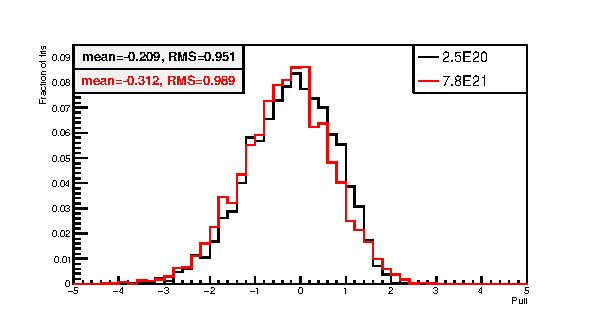
\includegraphics[width=\textwidth]{./images/fit_bias/pulls_rethrown/pull_f_skdetfsi005_rhc.eps}
  \label{fig:residuals:skdetfsi005}
  \caption{SuperK NC Normalisation}
 \end{subfigure}
 %
 \begin{subfigure}[b]{0.45\textwidth}
  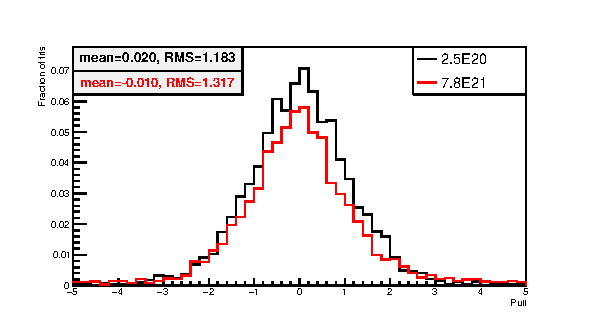
\includegraphics[width=\textwidth]{./images/fit_bias/pulls_rethrown/pull_f_sk_e_scale_rhc.eps}
  \label{fig:residuals:escale}
  \caption{SuperK Energy Scale}
 \end{subfigure}
 
 \caption {
      Distributions of pulls for four systematic parameters that have small biases. 
      These distributions are shown for both
      \FakePot{} POT (Runs 5 and 6, black histograms) and \TargetFullPot{} POT (the T2K ultimate goal, 
      red histograms).
  }
  \label{fig:residuals:badsystematics}
\end{figure*}


\begin{figure*}[htb]
  \center
  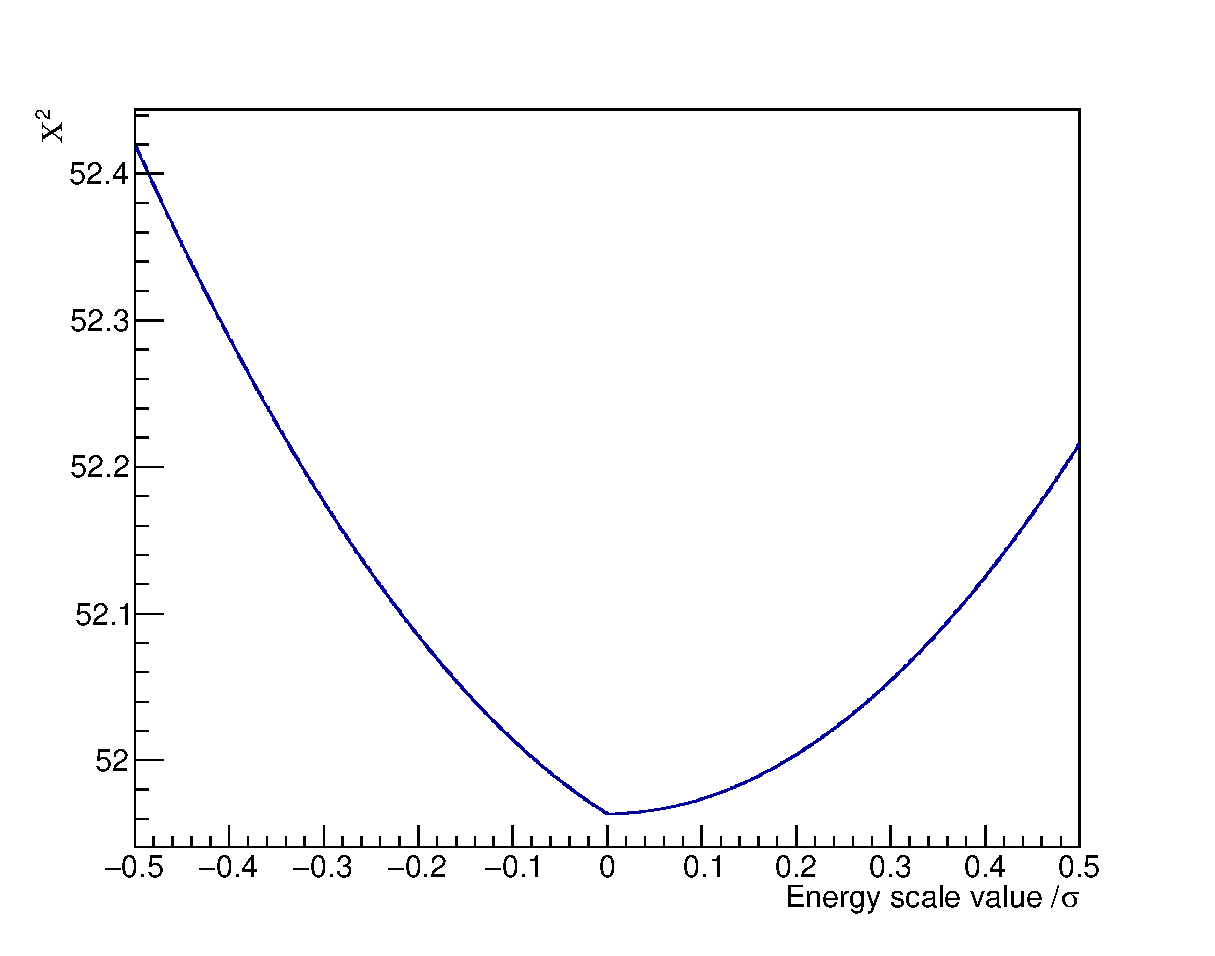
\includegraphics[width=30pc]{./images/fit_bias/energy_scale_chisquare_discontinuity.eps}
  \caption {
    The chi-square distribution when varying SuperK energy scale for a single randomised toy experiment.
    Note that the distribution is different on the two sides of the zero point, leading to
    a kink in the plot at zero.
    In the vast majority of datasets, this kink is imperceptible; the toy plotted here was selected
    specifically from our validation toys as a clear demonstration of the effect.
  }
  \label{fig:energy_scale_chisquare_discontinuity}
\end{figure*}
